\documentclass[10pt,a4paper,twocolumn]{jarticle}
%\documentclass[10pt,a4paper]{jarticle}
\usepackage{geometry}
\usepackage{pxchfon}
\usepackage{titlesec}
\usepackage{multicol}
\geometry{left=20mm,right=20mm,top=20mm,bottom=20mm}
\setlength{\columnsep}{10zw}
\usepackage{amssymb,amsmath,amsthm}
\usepackage{amsmath}
\usepackage[dvipdfmx]{graphicx}
\titleformat*{\section}{\normalsize}
\titleformat*{\subsection}{\normalsize}
\titleformat*{\subsubsection}{\normalsize}
\pagestyle{empty}
\renewcommand{\baselinestretch}{1.2}
\usepackage{multirow}
\usepackage{titlesec}
\makeatletter
\renewenvironment{thebibliography}[1]
{\section*{\refname\@mkboth{\refname}{\refname}}%
	\list{\@biblabel{\@arabic\c@enumiv}}%
	{\settowidth\labelwidth{\@biblabel{#1}}%
		\leftmargin\labelwidth
		\advance\leftmargin\labelsep
		\setlength\itemsep{0zh}%←ここの数値を調整(行間のつまり具合)
		\setlength\baselineskip{10pt}%←ここの数値を調整(追加)(文字の大きさ)
		\@openbib@code
		\usecounter{enumiv}%
		\let\p@enumiv\@empty
		\renewcommand\theenumiv{\@arabic\c@enumiv}}%
	\sloppy
	\clubpenalty4000
	\@clubpenalty\clubpenalty
	\widowpenalty4000%
	\sfcode`\.\@m}
{\def\@noitemerr
	{\@latex@warning{Empty `thebibliography' environment}}%
	\endlist}
\makeatother
\begin{document}
\twocolumn[
\begin{center}
{\large 卒業論文発表 要旨(2019年度版)\\
ワイヤレス給電システムの最適化のための能率的な動作周波数スイープ\\}
\end{center}
\begin{flushright}
	自動制御研究室\\
	森田 光流 \\
\end{flushright}
\vspace{\baselineskip}
]


\section{緒言}
ワイヤレス給電とはコネクタや金属接点の接触を用いず無線で電力を供給・伝搬することが可能な給電方法である.従来の電気製品の金属接点やコネクタを使用したものは水がかかると水による感電やショートをおこす,配線による転倒などの安全性に関して問題点がある.しかしワイヤレス給電は金属接点がないため前述の問題点を解決することができる.また非金属のものであればコイル間に存在していても送電側と受電側の電力に影響を及ぼさないため,人が立ち寄れない危険な場所や人体の中などにある機器や装置の遠隔操作ができるという点がある
\\ ワイヤレス給電の電力供給の効率の改善には色々と考えられているが本研究においては快適な周波数調整に注目し,最適動作周波数の探索することとした.最適動作周波数は高効率かつ大電力が出力される周波数である.その最適動作周波数探索するためには多くの周波数を測定しなければいけないので測定時間をなるべく短くしたい.しかし,ワイヤレス給電に周波数を送った後安定な電力が出力されるまで時間がかかる.したがって本研究は能率的な周波数スイープを設計し,ワイヤレス給電システムの最適動作周波数を能率的な周波数スイープによる測定・考察を目的とする.
\section{実験}
\subsection{実験回路}
\begin{figure}[h]
	\centering
	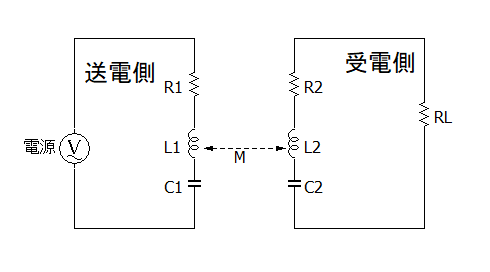
\includegraphics[scale=0.6]{wpt_2020128.png}
	\caption{ワイヤレス給電回路図}
	\label{fig:wpt_kairo}
\end{figure}
ワイヤレス給電は図\ref{fig:wpt_kairo}のように金属接点がない代わりに送電・受電にコイルを用いることにより,送電側の交流電源の電流が時間的に変化することにより受電側の磁束が変化しファラデーの電磁誘導の法則ににより誘導起電力が生じ誘導電流を伝えるという原理である.
なお本研究で使用した実験回路の素子の量は以下の表\ref{tab:para}ようになる.
\begin{table}[h]
	\centering
	\caption{実験回路パラメータ}
	\label{tab:para}
	\begin{tabular}{|l|l|l|}
		\hline
		パラメータ                          & 記号    & 値{[}単位{]}          \\ \hline
		\multirow{2}{*}{コイルの自己インダクタンス} & $L_1$ & $23.6[\mu H]$      \\ \cline{2-3} 
		& $L_1$ & $23.6[\mu H]$      \\ \hline
		相互インダクタンス                      & $M$   & $1.98[\mu H]$      \\ \hline
		\multirow{2}{*}{コイルの内部抵抗}      & $R_1$ & 0.08{[}$\Omega${]}  \\ \cline{2-3} 
		& $R_2$ & 0.08{[}$\Omega${]} \\ \hline
		負荷抵抗                           & $R_L$ & 25{[}$\Omega${]}   \\ \hline
	\end{tabular}
\end{table}
なお,実験回路の共振周波数は以下のとおりである.
\begin{equation}
f_0=99.7kHz \nonumber
\end{equation}

\subsection{周波数スイープ}
実験による最適動作周波数を探索する方法としては周波数スイープが挙げられる.周波数スイープとは一定の時間や速度において7周波数を変化させ出力させる方法である.なお本研究における周波数スイープのやり方でする.
\begin{enumerate}
	\item  一番最初の周波数を回路に送る.なお一番最初の周波数,一番最後の周波数,1つの周波数における測定時間,次の周波数で加算する周波数(以後加算周波数)の量をあらかじめ決めておく必要がある.
	\item 決めた時間で測定する.0.1秒ずつデータが出力される.
	\item 一定時間に達したら,加算周波数を加算し一番最後の周波数に達するまで繰り返す.
\end{enumerate}
 また,先行研究ではワイヤレス給電の周波数スイープをマイコンだけで実行したが,周波数を変更するにあたってわざわざコンパイルしなければならず面倒であった.そこで本研究では周波数スイープの周波数を送る・ワイヤレス給電の電力を受け取る作業をパソコンで自動化するようにした.
\subsection{最適動作判定}
ワイヤレス給電の最適動作周波数であるには前述にも述べたが高電力・高効率であることが重要である.したがって次の計算式(\ref{eq:saiteki})を導入した.なお定数はそれぞれ周波数スイープによって出力された受電側の電力$P_2$と送電側と受電側の出力結果を使って導き出された$効率\eta$である.
\begin{equation}
(最適動作判定)=P_2\eta
\label{eq:saiteki}
\end{equation}
\subsection{能率的な周波数スイープ}
先行研究では,ひとつの周波数を送って次の周波数送るまでの測定時間を10秒だった.しかし,本研究においては多くの周波数による電圧,電流,電力を測りたいがためあまり時間をかけたくない.また加算周波数を低周波数で設定すると確かに正確に測ることが可能だが時間がかかる.逆に大雑把に周波数を取りすぎると正確性に欠ける.したがって周波数スイープが能率的になる周波数の測定時間と,加算周波数の量を事前に決めておく必要がある.表\ref{tab:nouritu}は事前に決めた数値である.
\begin{table}[h]
	\centering

	\caption{測定時間・加速周波数決定値}
	\begin{tabular}{|l|l|}
		\hline
		測定時間  & 1.5s \\ \hline
		加算周波数 & 10k  \\ \hline
	\end{tabular}
\label{tab:nouritu}
\end{table}
\subsection{シミュレーション}
実験をする前に事前にシミュレートしてみた.図\ref{fig:simudousa}はそれぞれ電力出力,効率,最適動作判定の結果である.図\ref{fig:simudousa}からわかるとおり入力する周波数が共振周波数近くのとき最適動作周波数が最大だということが分かる.
\begin{figure}[h]
	\centering
	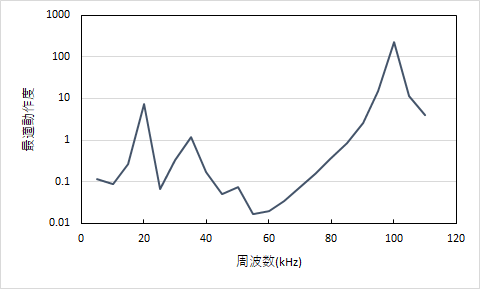
\includegraphics[scale=0.4]{saitekidousasimu.png}
	\caption{シミュレーションでの最適動作判定}
	\label{fig:simudousa}
\end{figure}
\section{実験結果・考察}
ここに能率的な動作周波数スイープと非能率の動作周波数スイープの実験結果をのせる.
\begin{figure}[h]
	\centering
	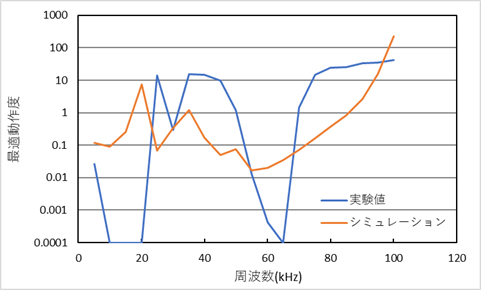
\includegraphics[scale=0.4]{simuhikaku.png}
	\caption{シミュレーションと実験結果との比較}
	\label{fig:simu-zitu}
\end{figure}
図\ref{fig:simu-zitu}からわかる通り出力結果にずれが生じていることが分かる.これは実験素子の実際の値が表\ref{tab:para}と比べてそれぞれ自己相互インダクタンス,コイルの内部抵抗,送電側受電側のコンデンサのずれが生じているから回路の共振周波数が変わりその結果電力の出力にずれが生じていると考えられる.
\vspace{\baselineskip}
\begin{figure}[h]
	\centering
	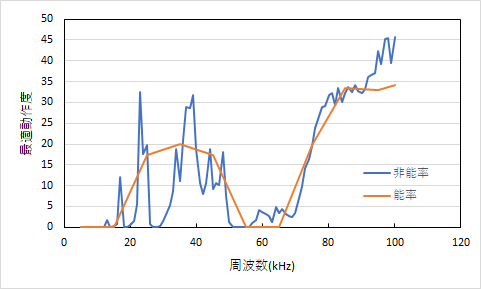
\includegraphics[scale=0.4]{nouritu-hinouritu.png}
	\caption{シミュレーションでの最適動作判定}
	\label{fig:nou-hinou}
\end{figure}
図\ref{fig:nou-hinou}からわかる通りどちらも最適な周波数の時最適動作度が大きくなっていることから最適動作周波数を見つけることができた.しかし非能率での測り方は先行研究と同じ計測時間である10秒間でかつ加算周波数の値が1kのため正確な値が出るが能率化した動作周波数スイープでは10$kHz$ずつ測っているため10kHz間での周波数変化に対応できていない.
\\ 改善点としては最適動作度の大きい範囲(図\ref{fig:nou-hinou}では$15kHzから45kHz$)を小さい加算周波数でまた測定するという方法が考えられるが時間がかかるという点が挙げられる.
\section{今後の方針}
能率的な周波数スイープを使うことにより,測定時間最短化することができた.それにより時間最短化することにより,ワイヤレス給電の状況によって周波数を変化させることにより受電側どんな状況にあってもいつも高電力を出力するように制御するということができると考えられる.しかし考察にもあるように非能率の周波数スイープと比べて正確性に欠ける.したがって正確かつ最短な能率的周波数スイープする方法を求められる.また,周波数スイープ以外による方法求められる.
\begin{thebibliography}{50}
	
	\bibitem{matuda}松田一志:”ワイヤレス給電システムのための電力測定回路の開発”,宮崎大学学士論文,平成30年度
	\bibitem{nakamura}中村裕馬:”ワイヤレス給電のための送電側100kHzプッシュプル回路”,宮崎大学学士論文,平成30年度
	\bibitem{rohm1}ローム株式会社:”ワイヤレス給電とは”ーエレクトロニクス豆知識, https://www.rohm.co.jp/electronics-basics/wireless-charging/wireless-charging\_what1,最終アクセス:2020/1/20
	\bibitem{rohm2}ローム株式会社:"ワイヤレス給電(無線給電)方式"ーエレクトロニクス豆知識, https://www.rohm.co.jp/electronics-basics/wireless-charging/wireless-charging\_what2
	\bibitem{goizuka}五位塚潤:"低周波数域駆動によるワイヤレス給電回路", 宮崎大学学士論文, 平成29年度
	\bibitem{hakugin}白銀聡一郎:"ワイヤレス給電のための短形波電源装置の設計と開発",宮崎大学学士論文,平成29年度
	\bibitem{morita}盛田穣文:"ワイヤレス給電システムの効率と電力の最適化について", 宮崎大学修士論文, 平成29年度
	\bibitem{ito}伊東雅浩:"短径波入力による高効率ワイヤレス給電の制御について", 宮崎大学修士論文, 平成30年度
	\bibitem{syourai}B\&PLUS:"ワイヤレス給電の現状と未来",https://www.b-plus-kk.jp/about/mechanism.html 最終アクセス:2020/1/23
	\bibitem{denki}電気の資格とお勉強:"RLC直列共振回路", https://eleking.net/study/s-accircuit/sac-resonant-rlcs.html 最終アクセス:2020/2/01
\end{thebibliography}
\end{document}
